\chapter{Existing Solutions}\label{sec-existing-solutions}

To improve the accuracy and reliability of software reverse engineering
techniques, numerous methods are proposed to tackle the challenges listed in
Chapter \ref{sec-challenges}.
Similarly, we follow the pipeline of software reverse engineering to introduce
these existing solutions.

\section{Disassembly} \label{sec:existing-disassembly}
As discussed in Chapter \ref{sec-challenges}, one of the major difficulties in
disassembly is differentiating code and data. While some successful disassembly
tools exist on the market~\cite{hex2014ida,kvroustek2017retdec,ghidra,radare},
these tools inevitably have substantial false positives (take data as code) and
false negatives (ignore code as data). In this section, we mainly discuss
several state-of-the-art disassembly and binary rewriting techniques that
solved the problem to a large extent.

\subsection{Superset Disassembly} \label{sec:existing-superset}
Bauman et al. proposed superset disassembly that employs the brute force
method to guarantee no false negatives~\cite{bauman2018superset}. To be more
specific, superset disassembly takes every offset in the text segment as one
possible start of an instruction, called superset instruction. It finds
intended sequences of instructions by brute force disassembling every possible
instruction, although the bytes of adjacent instructions may overlap.

As illustrated in \F~\ref{fig:superset}, the superset disassembly starts from
the offset $x$ and disassembles instructions until encountering an illegal
instruction (e.g., offset 3 and offset 5), then starts again from the offset
$x+1$. During disassembly, if the address of an instruction already appears in
a previous disassembly round that start from offset $y$, then a \textit{jmp}
instruction is added to transfer control flow to the disassembly result start
from offset $y$ to avoid unnecessary disassembly, e.g., this situation happens
from offsets 2 and 5 in \F~\ref{fig:superset}.

\begin{figure}[tb]
  \centering
  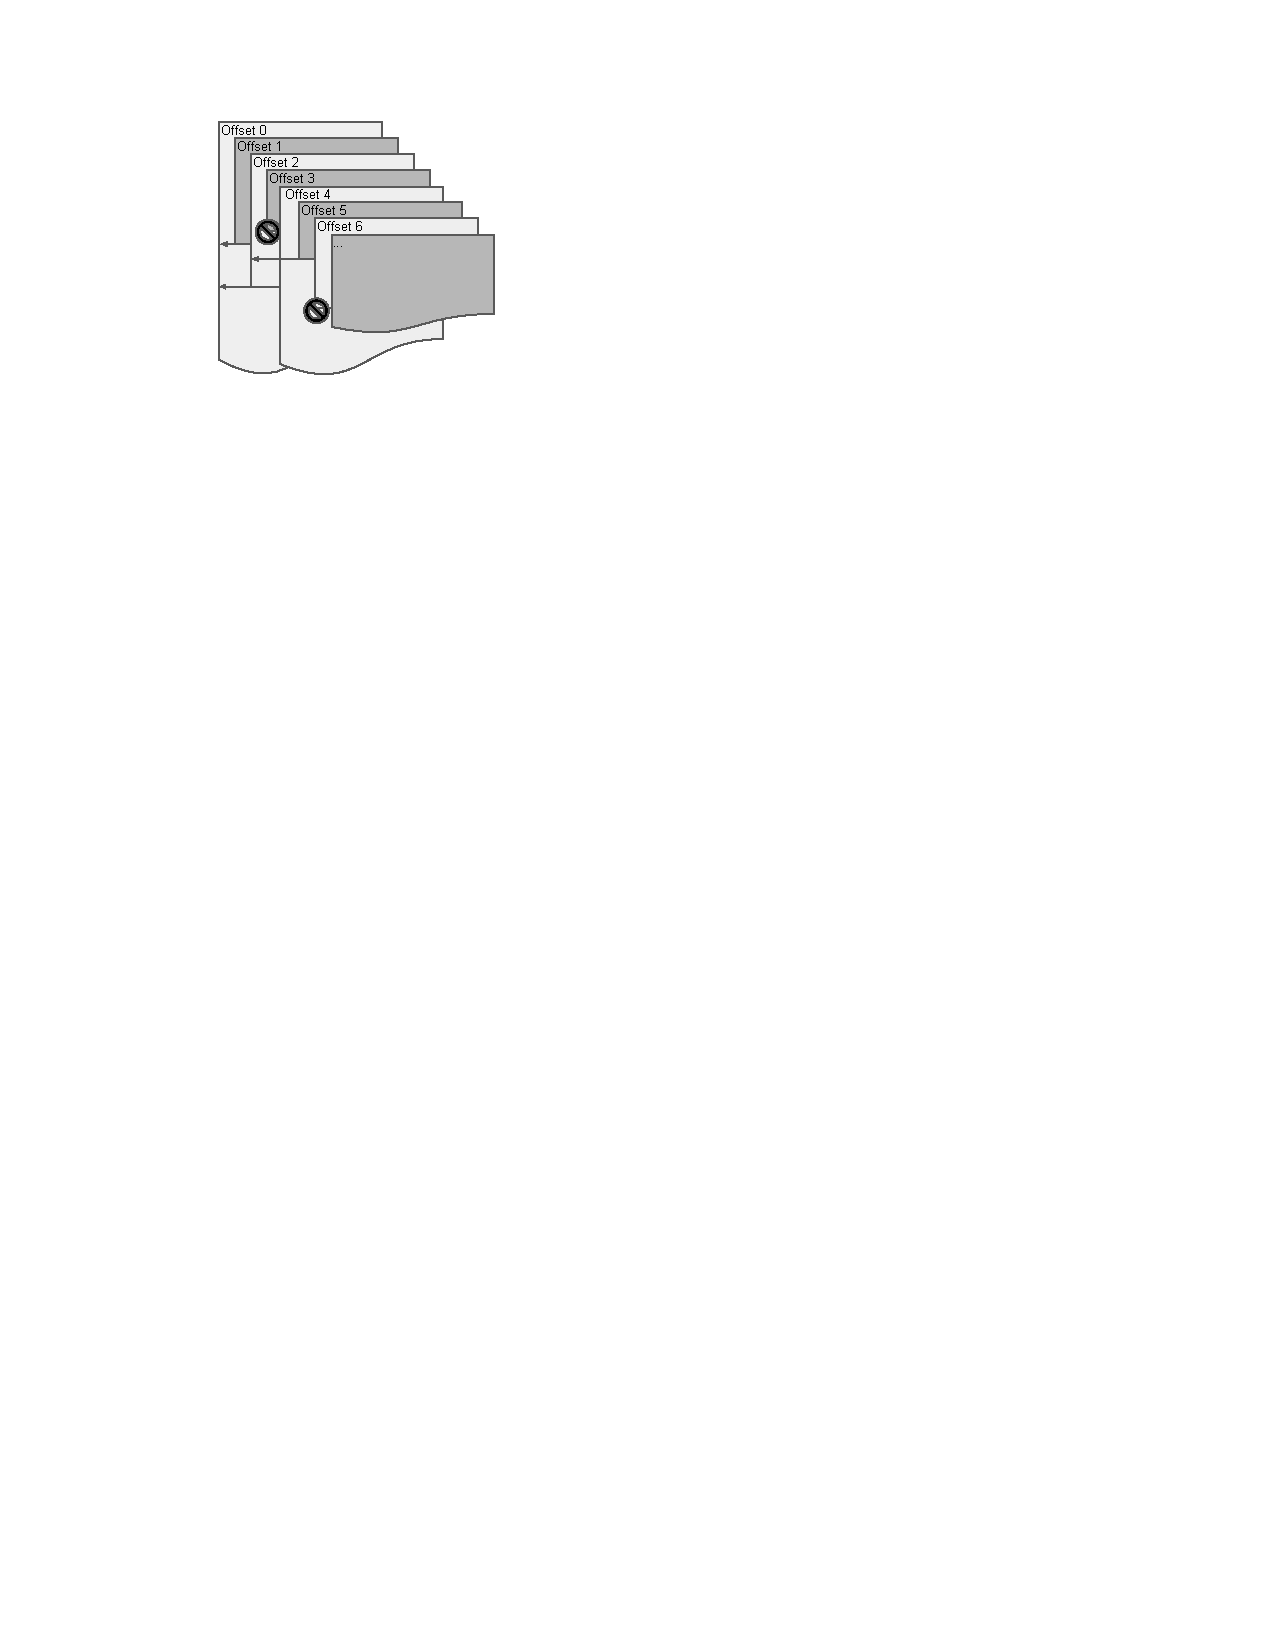
\includegraphics[width=0.4\textwidth]{fig/Superset-Disassembly.pdf}
  \caption{An illustration of superset disassembly strategy~\cite{bauman2018superset}.}
  \label{fig:superset}
\end{figure}

In this way, it can be guaranteed that there is no false positive in the
result, and thus enabling error-free binary rewriting (We will discuss how
superset disassembly addresses the symbolization problem in section
\fixme{XXX}). However, the disassembled program will be bloated as lots of
false-positive instructions exist. The bloated instructions could cause
substantial size and runtime overhead because getting the instruction to be
executed needs a table lookup each time, especially in practice, a binary writer based on superset disassembly has to instrument all superset instructions.

\subsection{Probabilistic Disassembly} \label{sec:existing-probabilistic}
Considering the size overhead and performance slowdown caused by superset
disassembly, Miller et al. proposed probabilistic disassembly based on superset
disassembly to reduce the number of false positives further. Probabilistic disassembly aims to reason the inherent uncertainty in the binary analysis due to the lack of debugging information. The basic idea is to compute the probabilities of each address being the true positive start of an instruction.

More explicitly, probabilistic disassembly defines three kind of hints, which are relations that imply true positive instructions:

\begin{itemize}

  \item \textbf{Hint \Romannum{1}: Control Flow Convergence.} Giving three instructions \textit{instr1}, \textit{instr2} and \textit{instr3}, where \textit{instr3} being the transfer target of \textit{instr1} and \textit{instr2} at the same time, as shown in \F~\hyperref[fig:hints]{1(a)}.
  \item \textbf{Hint \Romannum{2}: Control Flow Crossing.} Giving three instructions \textit{instr1}, \textit{instr2}, and \textit{instr3} follow \textit{instr2}, where \textit{instr3} is the target of \textit{instr1} and \textit{instr2} has a different target, as illustrated in \F~\hyperref[fig:hints]{1(b)}.
  \item \textbf{Hint \Romannum{3}: Register Define-use Relation.} todo

\end{itemize}

\begin{figure}[tb]
  \centering
  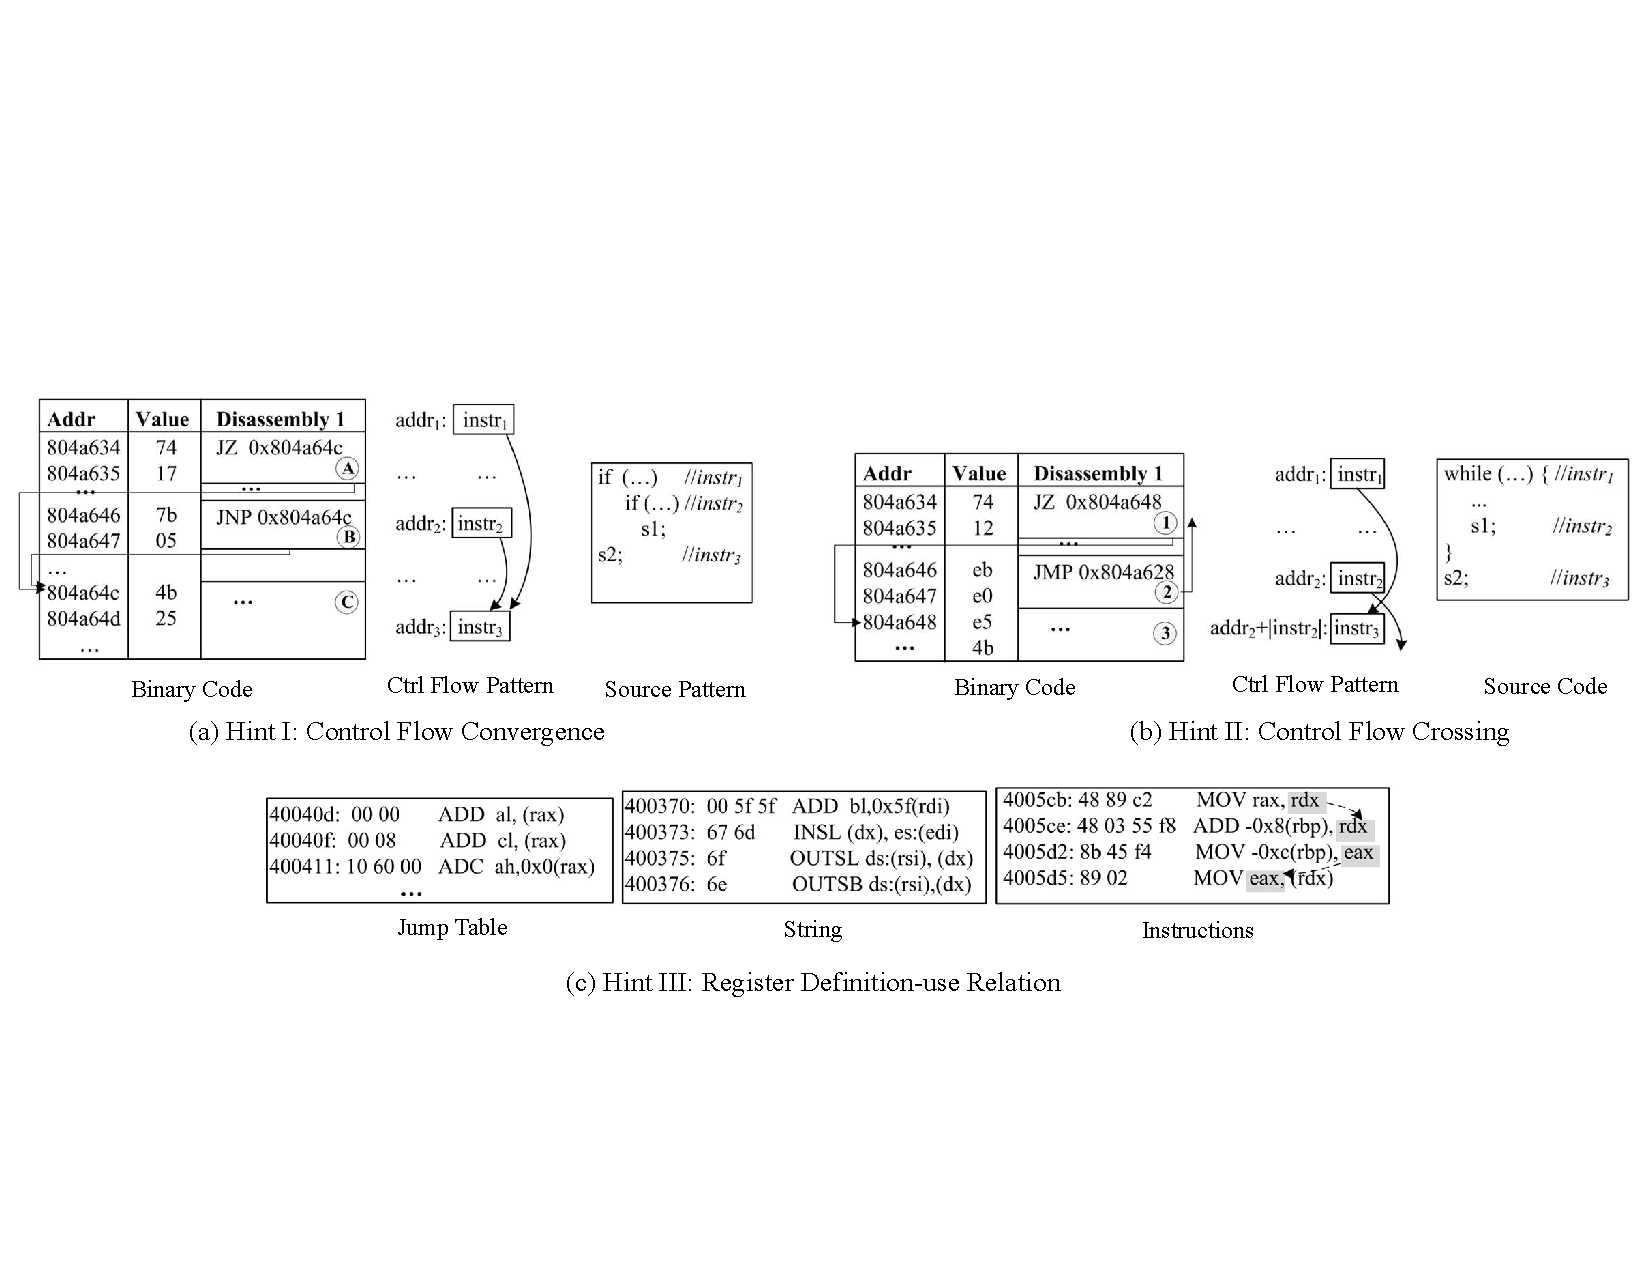
\includegraphics[width=1.0\textwidth]{fig/hints.pdf}
  \caption{An illustration of probabilistic disassembly hints~\cite{miller2019probabilistic}.}
  \label{fig:hints}
\end{figure}

\section{Lifting} \label{sec:existing-lifting}
TODO

\section{Decompilation} \label{sec:existing-decompilation}
TODO


\noindent\rule{8cm}{0.4pt}

\newpage
